\documentclass[12pt]{article}

\include{preamble}
\usepackage{amsmath}
\usepackage{amsmath, amssymb}

\newtoggle{professormode}
%\toggletrue{professormode} %STUDENTS: DELETE or COMMENT this line



\title{MATH 342W / 642 / RM742 Spring \the\year~HW \#2}

\author{Ye Htut Maung} %STUDENTS: write your name here

\iftoggle{professormode}{
\date{Due 11:59PM Feb 26 on github\\ \vspace{0.5cm} \small (this document last updated \currenttime~on \today)}
}

\renewcommand{\abstractname}{Instructions and Philosophy}

\begin{document}


\maketitle

\iftoggle{professormode}{
\begin{abstract}
The path to success in this class is to do many problems. Unlike other courses, exclusively doing reading(s) will not help. Coming to lecture is akin to watching workout videos; thinking about and solving problems on your own is the actual ``working out.''  Feel free to \qu{work out} with others; \textbf{I want you to work on this in groups.}

Reading is still \textit{required}. You should be googling and reading about all the concepts introduced in class online. This is your responsibility to supplement in-class with your own readings.

The problems below are color coded: \ingreen{green} problems are considered \textit{easy} and marked \qu{[easy]}; \inorange{yellow} problems are considered \textit{intermediate} and marked \qu{[harder]}, \inred{red} problems are considered \textit{difficult} and marked \qu{[difficult]} and \inpurple{purple} problems are extra credit. The \textit{easy} problems are intended to be ``giveaways'' if you went to class. Do as much as you can of the others; I expect you to at least attempt the \textit{difficult} problems. 

This homework is worth 100 points but the point distribution will not be determined until after the due date. See syllabus for the policy on late homework.

Up to 7 points are given as a bonus if the homework is typed using \LaTeX. Links to instaling \LaTeX~and program for compiling \LaTeX~is found on the syllabus. You are encouraged to use \url{overleaf.com}. If you are handing in homework this way, read the comments in the code; there are two lines to comment out and you should replace my name with yours and write your section. The easiest way to use overleaf is to copy the raw text from hwxx.tex and preamble.tex into two new overleaf tex files with the same name. If you are asked to make drawings, you can take a picture of your handwritten drawing and insert them as figures or leave space using the \qu{$\backslash$vspace} command and draw them in after printing or attach them stapled.

The document is available with spaces for you to write your answers. If not using \LaTeX, print this document and write in your answers. I do not accept homeworks which are \textit{not} on this printout. Keep this first page printed for your records.

\end{abstract}

\thispagestyle{empty}
\vspace{1cm}
NAME: \line(1,0){380}
\clearpage
}

\problem{These are questions about Silver's book, chapter 2, 3.  Answer the questions using notation from class (i.e. $t ,f, g, h^*, \delta, \epsilon, e, t, z_1, \ldots, z_t, \mathbb{D}, \mathcal{H}, \mathcal{A}, \mathcal{X}, \mathcal{Y}, X, y, n, p, x_{\cdot 1}, \ldots, x_{\cdot p}, x_{1 \cdot}, \ldots, x_{n \cdot}$, etc).}


\begin{enumerate}

\intermediatesubproblem{If one's goal is to fit a model for a phenomenon $y$, what is the difference between the approaches of the hedgehog and the fox? Connecting this to the modeling framework should really make you think about what Tetlock's observation means for political and historical phenomena.}\spc{3}

The difference between the approaches of the hedgehog and the fox is that since the hedgehogs only depend on one big idea or theory, when they are going to fit a model for a phenomenon $y$, they will only care about one main feature or a few of main features. Meanwhile, since the foxes rely on all the variables, features, diverse array of theories and they also change their perspective if they think that they are using the wrong technique. That is why when we predict about political and historical phenomena, their results are better when we care all the possible features for the model.

\easysubproblem{Why did Harry Truman like hedgehogs? Are there a lot of people that think this way?}\spc{2}

Harry Truman liked hedgebogs because the foxes in his administration couldn't give him an unqualified answer. Yes, there are a lot of people think this way. As an example, if you are politician and you only base on one big idea, people will like you because they think you are confident in what you are doing and many people think that kind of politician is correct. 

\hardsubproblem{Why is it that the more education one acquires, the less accurate one's predictions become?}\spc{3}

It is because when an individual is highly educated, they tend to overfit their models and analyses. They also information overloaded and so they will also account information that is not related to prediction and make them misjudgement.


\easysubproblem{Why are probabilistic classifiers (i.e. algorithms that output functions that return probabilities) better than vanilla classifiers (i.e. algorithms that only return the class label)? We will move in this direction in class soon.}\spc{4}

Probabilistic classifiers are better than vanilla classifiers because they can give you more insight about how much or how confident of the prediction of the class is correct or not. For example, the vanilla classifiers can give you the answer A but when we use probabilistic classifier, the probability of being answer A could be 50\% to 70\%. Moreover, when the new data comes in, it can help to refine accuracy over time which is more efficient compared to training model again for vanilla classifier.


\easysubproblem{What algorithm that we studied in class is PECOTA most similar to?}\spc{1}

The k nearest neighbors algorithm is the algorithm that we studied in class which is PECOTA most similar to.

\easysubproblem{Is baseball performance as a function of age a linear model? Discuss.}\spc{4}

No, it is not a linear model.  Baseball players typically imporve until their late twenties. The average age of the peak performance of the baseball players is 27. Then, the performance gradually decline in their thirties. 

\intermediatesubproblem{How can baseball scouts do better than a prediction system like PECOTA?}\spc{6}

Baseball scouts can do better than a prediction system like PECOTA by directly observing a player's mechanics, speed and strength. They can also adjust information in real time whereas PECOTA needs to wait for a full season for the data to be updated. They also have better access to data as they can just find the information by measuring in real time.


\intermediatesubproblem{Why hasn't anyone (at the time of the writing of Silver's book) taken advantage of Pitch f/x data to predict future success?}\spc{6}

No one has taken advantage of Pitch f/x data to predict future success because it is a new technology which can measure many data in 3 dimensional space and there are so many data about how pitcher throw a ball, vertically and horizontally and other data. Since those are the new data, there might now enough historical data to be able to train a good model. It is also difficult to choose which information is crucial for prediction since more information do not mean more good data. 


\end{enumerate}



\problem{These are questions about the SVM.}

\begin{enumerate}

\easysubproblem{State the hypothesis set $\mathcal{H}$ inputted into the support vector machine algorithm. Is it different than the $\mathcal{H}$ used for $\mathcal{A}$ = perceptron learning algorithm?}\spc{1}

\[
H = \left\{ \mathbb{1} \left( \mathbf{w} \cdot \mathbf{x} - b \geq 0 \right) \mid \mathbf{w} \in \mathbb{R}^p, b \in \mathbb{R} \right\}
\]

It is similar to $\mathcal{H}$ used for $\mathcal{A}$ = perceptron learning algorithm.


\extracreditsubproblem{Prove the max-margin linearly separable SVM converges. State all assumptions. Write it on a separate page.}\spc{-0.5}

\hardsubproblem{Let $\mathcal{Y} = \braces{-1,1}$. Rederive the cost function whose minimization yields the SVM line in the linearly separable case. }\spc{20}

\[ \mathcal{Y} = \{-1,1\} \]

All \( y = 1 \)'s are above or equal to \( l_U \)

\[ \forall i \text{ such that } y_i = 1, \quad \mathbf{w'} \cdot \mathbf{x}_i - (b' + 1) \geq 0 \]
\[ \mathbf{w'} \cdot \mathbf{x}_i - b' - 1 \geq 0 \]
\[ \mathbf{w'} \cdot \mathbf{x}_i - b' \geq 1 \]
\[ y_i (\mathbf{w'} \cdot \mathbf{x}_i - b') \geq 1 \]

All \( y = -1 \)'s are below or equal to \( l_L \)

\[ \forall i \text{ such that } y_i = -1, \quad \mathbf{w'} \cdot \mathbf{x}_i - (b' - 1) \leq 0 \]
\[ \mathbf{w'} \cdot \mathbf{x}_i - b' + 1 \leq 0 \]
\[ \mathbf{w'} \cdot \mathbf{x}_i - b' \leq -1 \]
\[ - (\mathbf{w'} \cdot \mathbf{x}_i - b') \geq 1 \]
\[ y_i (\mathbf{w'} \cdot \mathbf{x}_i - b') \geq 1 \]

Thus, the inequality holds for all \( i \):
\[ y_i (\mathbf{w'} \cdot \mathbf{x}_i - b') \geq 1 \]

If \( y_i (\mathbf{w'} \cdot \mathbf{x}_i - b') < 1 \), then there is an error.

\[ y_i (\mathbf{w'} \cdot \mathbf{x}_i - b') = 1 - d_i \]

\[ d_i = 1 - (y_i (\mathbf{w'} \cdot \mathbf{x}_i - b')) \]

\( d_i \) represents the severity of the error, and the hinge loss function is:
\[ H_i = \max{0,d_i}\]

The sum of hinge errors (SHE) is defined as:
\[ SHE = \sum_{i=1}^{n} \max { 0, d_i } \]
\[ SHE= \sum_{i=1}^{n} \max{ 0, 1 - (y_i (\mathbf{w'} \cdot \mathbf{x}_i - b'))} \]


\easysubproblem{Given your answer to (c) rederive the cost function using the \qu{soft margin} i.e. the hinge loss plus the term with the hyperparameter $\lambda$. This is marked easy since there is just one change from the expression given in class.}\spc{4}


\[ \mathbf{w}^*, b^* = \argmin_{\mathbf{w'} \in \mathbb{R}^p, b \in \mathbb{R}} \left\{ \frac{1}{n} \sum_{i=1}^{n} \max{ 0, 1 - (y_i (\mathbf{w'} \cdot \mathbf{x}_i - b'))} + \lambda \|\mathbf{w'}\| \right\} \]



\end{enumerate}



\problem{These are questions are about the $k$ nearest neighbors (KNN) algorithm.}

\begin{enumerate}

\easysubproblem{Describe how the algorithm works. Is $k$ a \qu{hyperparameter}?}\spc{5}

We use $k$ nearest neighbors algorithm when the classification is more than 2 (not binary classification). The algorithm works by choosing k numbers of data points and when there is a new data, they find the distance between the new data and k numbers of historical data. Then, they sort the distance and the category of the most shortest distance will be assigned to the new data. Yes, $k$ is a \qu{hyperparameter}.

\hardsubproblem{[MA] Assuming $\mathcal{A} = $ KNN, describe the input $\mathcal{H}$ as best as you can.}\spc{8}

When I research about Hypothesis set for KNN, I found the \href{https://sebastianraschka.com/pdf/lecture-notes/stat479fs18/02_knn_notes.pdf}{lecture note} from University of Wisconsin\_Madison. I did not add the formula for finding the distance between two data points. 

The delta function will return how many time of a specfic class will be found among the nearest neighbors. Then, add all the occurrence and return the maximum number of occurrence class.


\[
\mathcal{H}(\mathbf{x}^{[q]}) = \argmax\limits_{y \in \{1, \dots, t\}} \sum_{i=1}^{k} \delta(y, f(\mathbf{x}^{[i]})).
\]


\[
\delta(a, b) =
\begin{cases}
1, & \text{if } a = b, \\
0, & \text{if } a \neq b.
\end{cases}
\]




\easysubproblem{When predicting on $\mathbb{D}$ with $k=1$, why should there be zero error? Is this a good estimate of future error when new data comes in? (Error in the future is called \emph{generalization error} and we will be discussing this later in the semester).}\spc{5}

When predicting on $\mathbb{D}$ with $k = 1$, there should be zero error because you only find the distance of one nearest data and not comparing wiht other data points. So, when you train the model, there will be zero error. This is not a good estimate of future error when new data comes in because this model is overfitting and it does not generalize well to make a good prediction of the future data.

\end{enumerate}

\problem{These are questions about the linear model with $p=1$.}

\begin{enumerate}

\easysubproblem{What does $\mathbb{D}$ look like in the linear model with $p=1$? What is $\mathcal{X}$? What is $\mathcal{Y}$?}\spc{3}

$\mathbb{D}$ looks like a pair of ($x_i$, $y_i$) with $n$ rows. $\mathcal{X}$ = $\mathbb{R}$ and $\mathcal{Y}$ = $\mathbb{R}$


\easysubproblem{Consider the line fit using the ordinary least squares (OLS) algorithm. Prove that the point $<\xbar, \ybar>$ is on this line. Use the formulas we derived in class.}\spc{3}

Given the point \(< \bar{x}, \bar{y} > \), the function \( g(x) \) represents the fitted line using Ordinary Least Squares (OLS):

\[
g(x_*) = b_0 + b_1 x_*
\]

Evaluating at \( \bar{x} \):

\[
g(\bar{x}) = b_0 + b_1 \bar{x}
\]

By substituting \(b_0 = \bar{y} - b_1 \bar{x} \):

\[
g(\bar{x}) = \bar{y} - b_1 \bar{x} + b_1 \bar{x}
\]

\[
g(\bar{x}) = \bar{y}
\]

Therefore, the point \( \langle \bar{x}, \bar{y} \rangle \) is always on the line produced by the OLS algorithm.



\intermediatesubproblem{Consider the line fit using OLS. Prove that the average prediction $\hat{y}_i := g(x_i)$ for $x_i \in \mathbb{D}$ is $\ybar$.}\spc{4}

Average prediction:

\[
\frac{1}{n} \sum_{i=1}^{n} \hat{y}_i
\]

\[
\frac{1}{n} \sum_{i=1}^{n} \hat{y}_i = \frac{1}{n} \sum_{i=1}^{n} (b_0 + b_1 x_i)
\]

\[
= \frac{1}{n} \cdot n \cdot b_0 + b_1 \cdot \frac{1}{n} \sum_{i=1}^{n} x_i
\]

\[
= b_0 + b_1 \bar{x}
\]

\[
= \bar{y} - b_1 \bar{x} + b_1 \bar{x}
\]

\[
\frac{1}{n} \sum_{i=1}^{n} \hat{y}_i = \bar{y}
\]


\intermediatesubproblem{Consider the line fit using OLS. Prove that the average residual $e_i$ is 0 over $\mathbb{D}$.}\spc{6}

\[
\sum_{i=1}^{n} e_i = \sum_{i=1}^{n} (y_i - \hat{y}_i) = \sum_{i=1}^{n} y_i - \sum_{i=1}^{n} (b_0 + b_1 x_i)
\]

\[
= \sum_{i=1}^{n} y_i - \sum_{i=1}^{n} b_0 - \sum_{i=1}^{n} b_1 x_i
\]

\[
= n\bar{y} - n b_0 - b_1 n\bar{x}
\]

Substituting \( b_0 \):

\[
= n\bar{y} - n (\bar{y} - b_1 \bar{x}) - n b_1 \bar{x}
\]

\[
= n\bar{y} - n\bar{y} + n b_1 \bar{x} - n b_1 \bar{x} = 0
\]

\[
\sum_{i=1}^{n} e_i = 0
\]

Therefore, multiply both side by $\frac{1}{n}$:

\[
\frac{1}{n} \sum_{i=1}^{n} e_i = 0
\]

\[
\bar{e} = 0
\]


\intermediatesubproblem{Why is the RMSE usually a better indicator of predictive performance than $R^2$? Discuss in English.}\spc{4}

The RMSE is usually a better indicator of predictive performance than $R^2$ because $R^2$ can be very high like 0.99 but RMSE can still be too large to be useful. For example, you are predicting the supermarket sale and the prediction is about \$300 million sale. The $R^2$ is 0.90 which is pretty good. However, the RMSE can be like \$30-50 million or more which is a lot. So, we can't trust $R^2$ only and we also need to consider RMSE.


\intermediatesubproblem{$R^2$ is commonly interpreted as \qu{proportion of the variance explained by the model} and proportions are constrained to the interval $\zeroonecl$. While it is true that $R^2 \leq 1$ for all models, it is not true that $R^2 \geq 0$ for all models. Construct an explicit example $\mathbb{D}$ and create a linear model $g(x) = w_0 + w_1 x$ whose $R^2 < 0$.}\spc{10}

It can be less than 0 because when SSE is greater than SST which mean, the error of the predicted model is greater than the error of the null model. When this occurs, your model is worse than the null or naive model. The following is showing how to get $R^2$ using specific $\mathbb{D}$ and specific linear model. Let $\mathbb{D}$ be {(1,4),(2,5),(3,3),(4,3),(5,5),(6,4)}. 

\[
\bar{y} = \frac{4 + 5 + 3 + 3 + 5 + 4}{6} = \frac{24}{6} = 4.
\]

Computer SST:

\[
\text{SST} = \sum_{i=1}^{6} (y_i - \bar{y})^2
\]

\[
= (4 - 4)^2 + (5 - 4)^2 + (3 - 4)^2 + (3 - 4)^2 + (5 - 4)^2 + (4 - 4)^2
\]

\[
= 0 + 1 + 1 + 1 + 1 + 0 = 4.
\]

Choose the linear model:

\[
g(x) = 6 - 2x.
\]

For each \( x \):

\[
\begin{aligned}
g(1) &= 6 - 2(1) = 4, \\
g(2) &= 6 - 2(2) = 2, \\
g(3) &= 6 - 2(3) = 0, \\
g(4) &= 6 - 2(4) = -2, \\
g(5) &= 6 - 2(5) = -4, \\
g(6) &= 6 - 2(6) = -6.
\end{aligned}
\]

Compute SSE:

\[
\text{SSE} = \sum_{i=1}^{6} (y_i - g(x_i))^2
\]

\[
= (4 - 4)^2 + (5 - 2)^2 + (3 - 0)^2 + (3 - (-2))^2 + (5 - (-4))^2 + (4 - (-6))^2
\]

\[
= 0^2 + 3^2 + 3^2 + 5^2 + 9^2 + 10^2
\]

\[
= 0 + 9 + 9 + 25 + 81 + 100 = 224.
\]

Compute \(R^2\):

\[
R^2 = 1 - \frac{\text{SSE}}{\text{SST}}
\]

\[
= 1 - \frac{224}{4} = 1 - 56 = -55.
\]

\hardsubproblem{You are given $\mathbb{D}$ with $n$ training points $<x_i, y_i>$ but now you are also given a set of weights $\bracks{w_1~w_2~ \ldots ~w_n}$ which indicate how costly the error is for each of the $i$ points. Rederive the least squares estimates $b_0$ and $b_1$ under this situation. Note that these estimates are called the \emph{weighted least squares regression} estimates. This variant $\mathcal{A}$ on OLS has a number of practical uses, especially in Economics. No need to simplify your answers like I did in class (i.e. you can leave in ugly sums).}\spc{12.5}


Minimize the weighted sum of squared errors (SSE):

\[
SSE = \sum_{i=1}^{n} w_i e_i^2.
\]

\[
= \sum_{i=1}^{n} w_i (y_i - \hat{y})^2.
\]

\[
SSE = \sum_{i=1}^{n} w_i (y_i - b_0 - b_1 x_i)^2.
\]



\[
\frac{\partial}{\partial b_0} [SSE] = -2 \sum_{i=1}^{n} w_i (y_i - b_0 - b_1 x_i).
\]

Setting this equal to zero:

\[
0 = \sum_{i=1}^{n} w_i y_i - b_0 \sum_{i=1}^{n} w_i - b_1 \sum_{i=1}^{n} w_i x_i.
\]

Defining the weighted means:

\[
\bar{x}_w = \frac{\sum_{i=1}^{n} w_i x_i}{\sum_{i=1}^{n} w_i}, \quad
\bar{y}_w = \frac{\sum_{i=1}^{n} w_i y_i}{\sum_{i=1}^{n} w_i}.
\]

Rearrange:

\[
b_0 + b_1 \frac{\sum_{i=1}^{n} w_i x_i}{\sum_{i=1}^{n} w_i} = \frac{\sum_{i=1}^{n} w_i y_i}{\sum_{i=1}^{n} w_i}.
\]

\[
b_0 + b_1 \bar{x}_w = \bar{y}_w.
\]

Solving for \( b_0 \):

\[
b_0 = \bar{y}_w - b_1 \bar{x}_w.
\]

Derivative with respect to \( b_1 \)
\[
\frac{\partial}{\partial b_1} [SSE] = \frac{\partial}{\partial b_1} \sum_{i=1}^{n} w_i (y_i - b_0 - b_1 x_i)^2
\]

\[
= \sum_{i=1}^{n} -2 w_i x_i (y_i - b_0 - b_1 x_i).
\]

Expanding:

\[
= -2 \sum_{i=1}^{n} w_i x_i y_i + 2 b_0 \sum_{i=1}^{n} w_i x_i + 2 b_1 \sum_{i=1}^{n} w_i x_i^2.
\]

Setting this to zero:

\[
\sum_{i=1}^{n} w_i x_i y_i = b_0 \sum_{i=1}^{n} w_i x_i + b_1 \sum_{i=1}^{n} w_i x_i^2.
\]

Solving for \( b_1 \):

\[
b_1 = \frac{\sum_{i=1}^{n} w_i x_i y_i - \bar{y}_w \sum_{i=1}^{n} w_i x_i}{\sum_{i=1}^{n} w_i x_i^2 - \bar{x}_w \sum_{i=1}^{n} w_i x_i}.
\]

Answer:
 
\[
b_0 = \bar{y}_w - b_1 \bar{x}_w.
\]

\[
b_1 = \frac{\sum_{i=1}^{n} w_i x_i y_i - \bar{y}_w \sum_{i=1}^{n} w_i x_i}{\sum_{i=1}^{n} w_i x_i^2 - \bar{x}_w \sum_{i=1}^{n} w_i x_i}.
\]


\intermediatesubproblem{Interpret the ugly sums in the $b_0$ and $b_1$ you derived above and compare them to the $b_0$ and $b_1$ estimates in OLS. Does it make sense each term should be altered in this matter given your goal in the weighted least squares?}\spc{5}

In OLS, the means \( \bar{x} \) and \( \bar{y} \) are simple arithmetic means.

In WLS, the means \( \bar{x}_w \) and \( \bar{y}_w \) are weighted averages, giving more influence to data points with higher weights.

Yes, It makes sense.


%\hardsubproblem{[MA] In class we talked about $x_{raw} \in \braces{\text{red}, \text{green}}$ and the OLS model was the sample average of the inputted $x$ where $b_0 = \ybar_r$ and $b_1 = \ybar_g - \ybar_r$. Reparameterize $\mathcal{H} = \braces{w_1\indic{x_{raw} =~\text{red}}  + w_2 \indic{x_{raw} =~\text{green}}~:~ w_1, w_2 \in \reals}$ and prove that the OLS estimates are $b_1 = \ybar_r$ and $b_2 = \ybar_g$.}\spc{20}

\extracreditsubproblem{In class we talked about $x_{raw} \in \braces{\text{red}, \text{green}}$ and the OLS model was the sample average of the inputted $x$. Imagine if you have the additional constraint that $x_{raw}$ is ordinal e.g. $x_{raw} \in \braces{\text{low}, \text{high}}$ and you were forced to have a model where $g$(low) $\leq$ $g$(high). Write about an algorithm $\mathcal{A}$ that can solve this problem.}\spc{10}

\end{enumerate}

\problem{These are questions about association and correlation.}


\begin{enumerate}

\easysubproblem{Give an example of two variables that are both correlated and associated by drawing a plot.}\spc{7}

\begin{figure}[H]
    \centering
    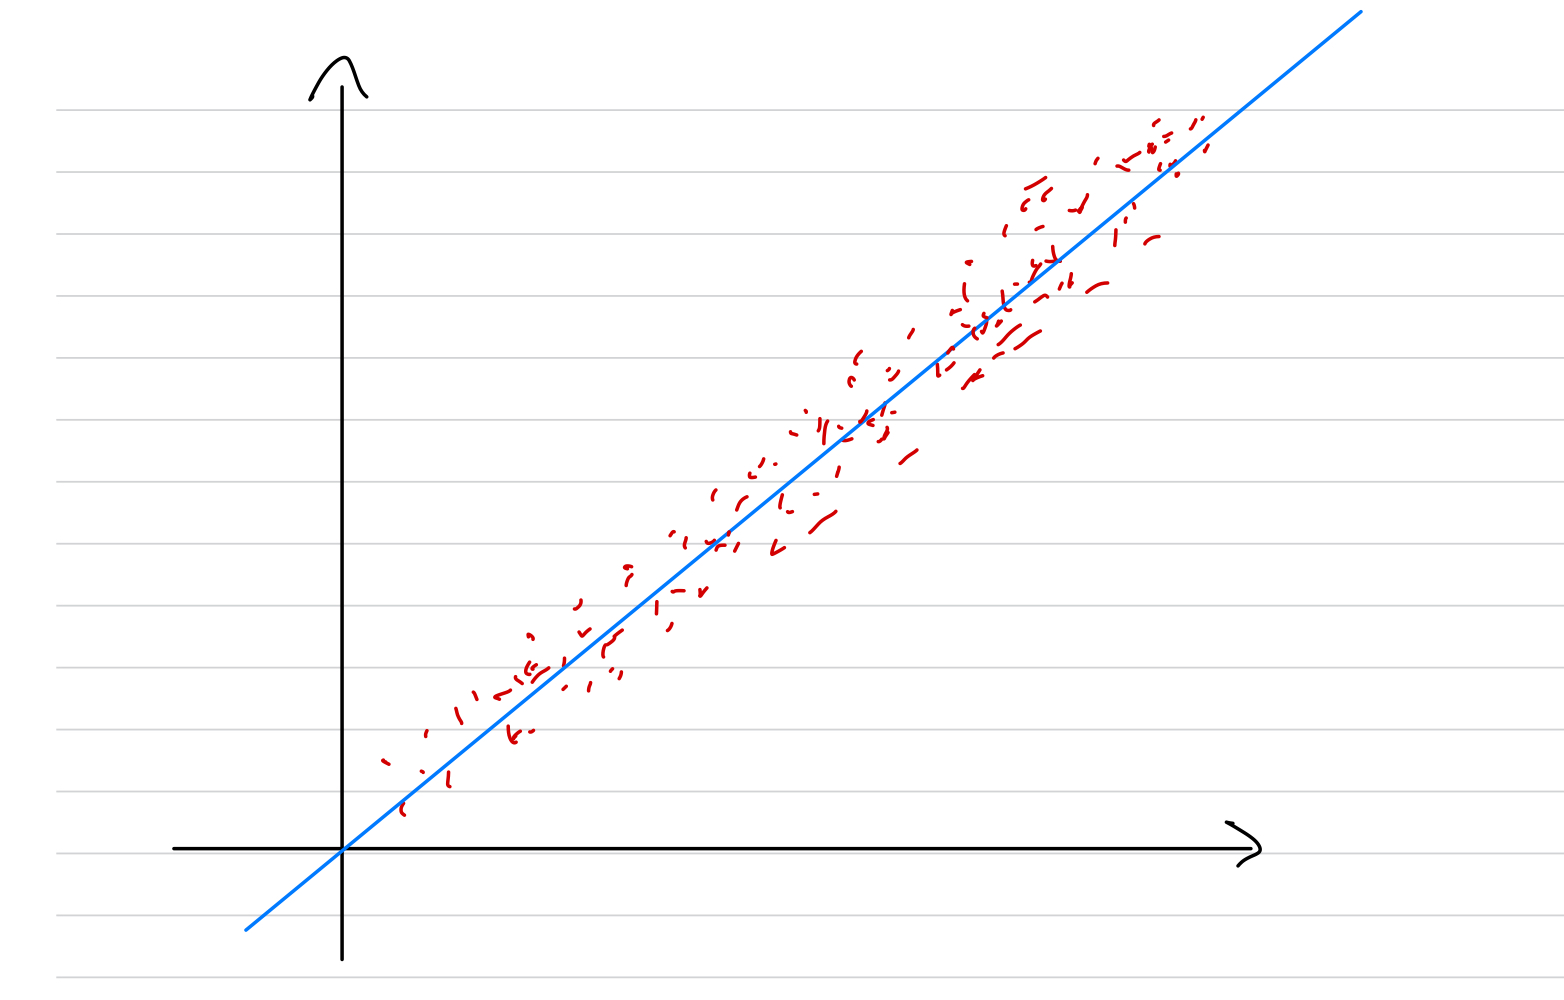
\includegraphics[width=0.75\linewidth]{img1 p5.jpeg}
    \caption{Both Correlated and Associated Figure}
    \label{fig:enter-label}
\end{figure}


When two variables are associated, there is a pattern in the coordinate plane. Those two variables are not scatter around the plane. When two variables are correlated, there is a linear trend which also need to be associated because correlation is a specific form of association. For example, Students who spend more time studying tend to score higher on exams. The amount of time spend studying is on the X-axis and the score they got is on the Y-axis

\easysubproblem{Give an example of two variables that are not correlated but are associated by drawing a plot.}\spc{7}

\begin{figure}[H]
    \centering
    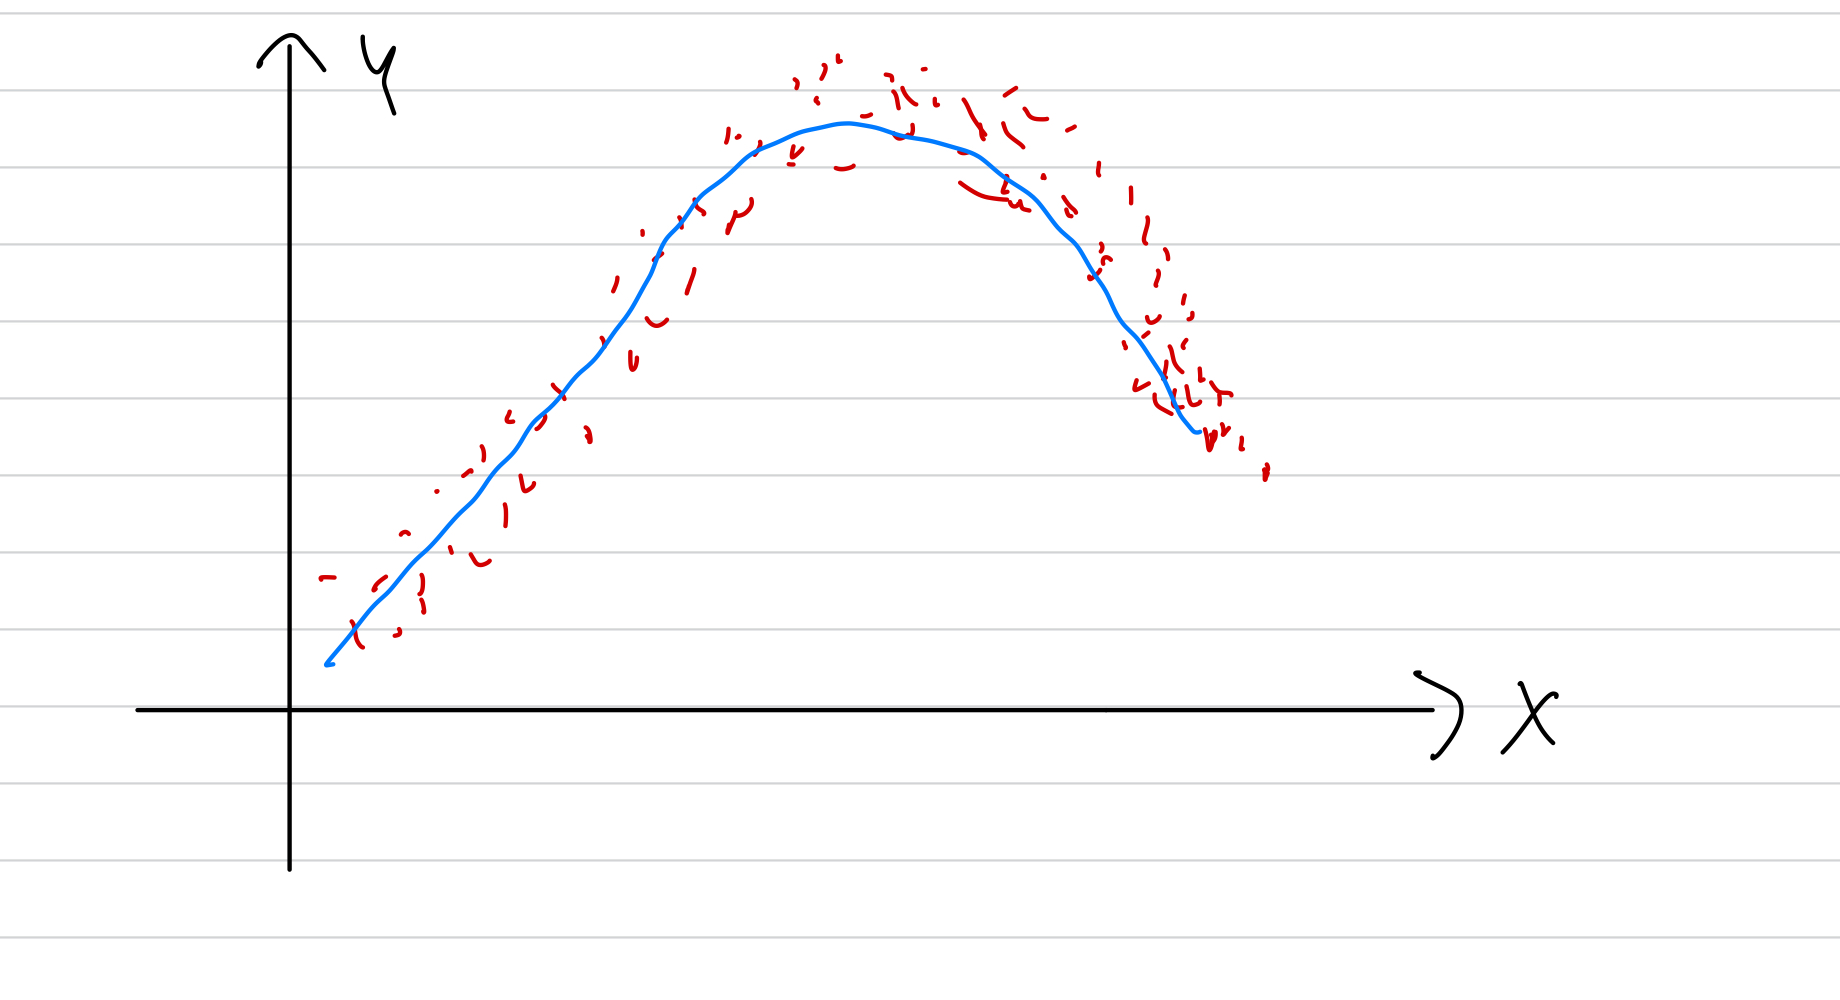
\includegraphics[width=0.75\linewidth]{img2 p5.jpeg}
    \caption{Not Correlated but are Associated Figure}
    \label{fig:enter-label}
\end{figure}

Correlation needs to be a linear trend but this is a polynoimal curve. However, you can see the pattern in the figure formed by the data points. This figure is the example of temperature throughout the day. From 12AM to 11:59PM. The temperature is low and it is increasing during the day and decreasing during evening.

\easysubproblem{Give an example of two variables that are not correlated nor associated by drawing a plot.}\spc{7}

\begin{figure}[H]
    \centering
    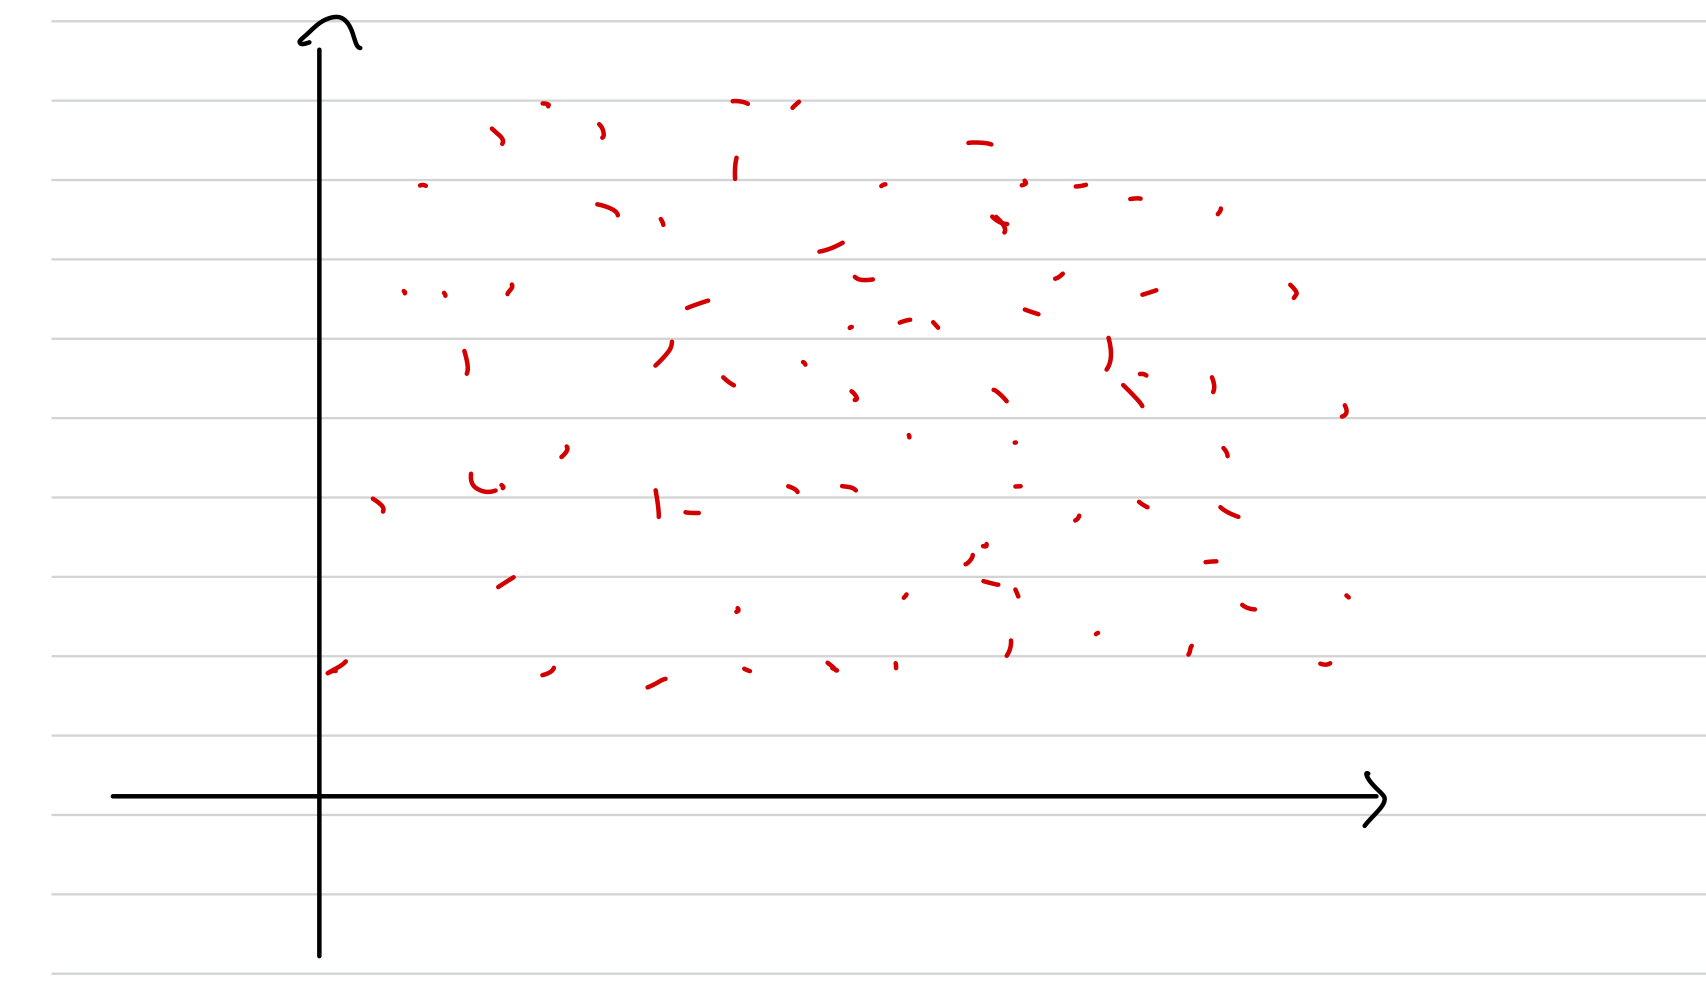
\includegraphics[width=0.75\linewidth]{img3 p5.jpeg}
    \caption{Not Correlated nor Associated Figure}
    \label{fig:enter-label}
\end{figure}

Not correlated nor associated means that there is not pattern or linear trend in the picture or data points when you draw. The data points are all scatter around the coordinate plane. This is an example of the number of shoes a person owns and the number of a person owns. It has not association between those two.

\easysubproblem{Can two variables be correlated but not associated? Explain.}\spc{7}

No. Two variables cannot be correlated but not associated because correlation is a specific condition of association. If there is no association, there will never be correlation bewteeen two variables.

\end{enumerate}


\problem{These are questions about multivariate linear model fitting using the least squares algorithm.}

\begin{enumerate}

\hardsubproblem{Derive $\partialop{\c}{\c^\top A \c}$ where $\c \in \reals^n$ and $A \in \reals^{n \times n}$ but \textit{not} symmetric. Get as far as you can.}\spc{8}

\easysubproblem{Given matrix $X \in \reals^{n \times (p+1)}$, full rank and first column consisting of the $\onevec_n$ vector, rederive the least squares solution $\b$ (the vector of coefficients in the linear model shipped in the prediction function $g$). No need to rederive the facts about vector derivatives.}\spc{10}

\begin{figure}[H]
    \centering
    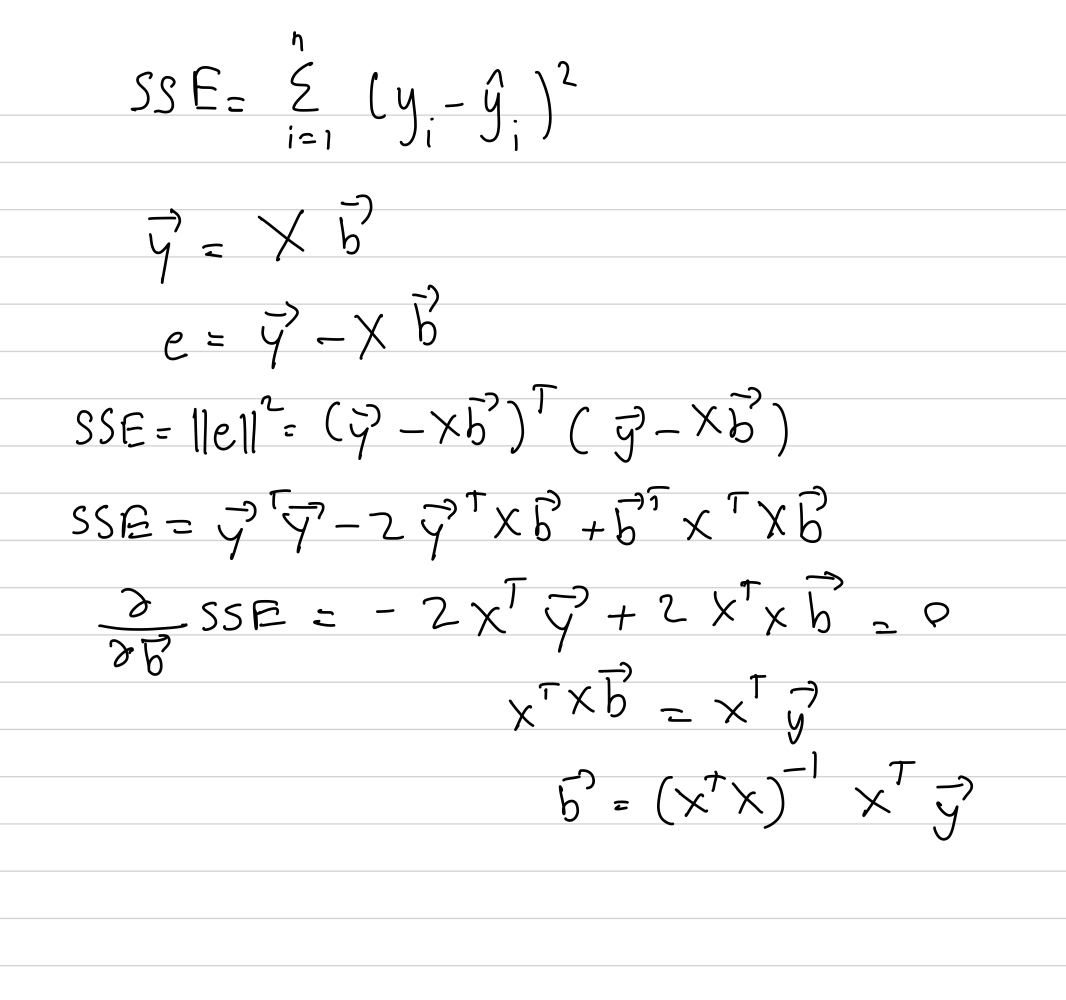
\includegraphics[width=0.75\linewidth]{IMG_8C8D025D366B-1.jpeg}
    \caption{Problem 6(b)}
    \label{fig:enter-label}
\end{figure}

\intermediatesubproblem{Consider the case where $p = 1$. Show that the solution for $\b$ you just derived in (b) is the same solution that we proved for simple regression. That is, the first element of $\b$ is the same as $b_0 = \ybar - r \frac{s_y}{s_x}\xbar$ and the second element of $\b$ is $b_1 = r \frac{s_y}{s_x}$.} \spc{7}

\begin{figure}[H]
    \centering
    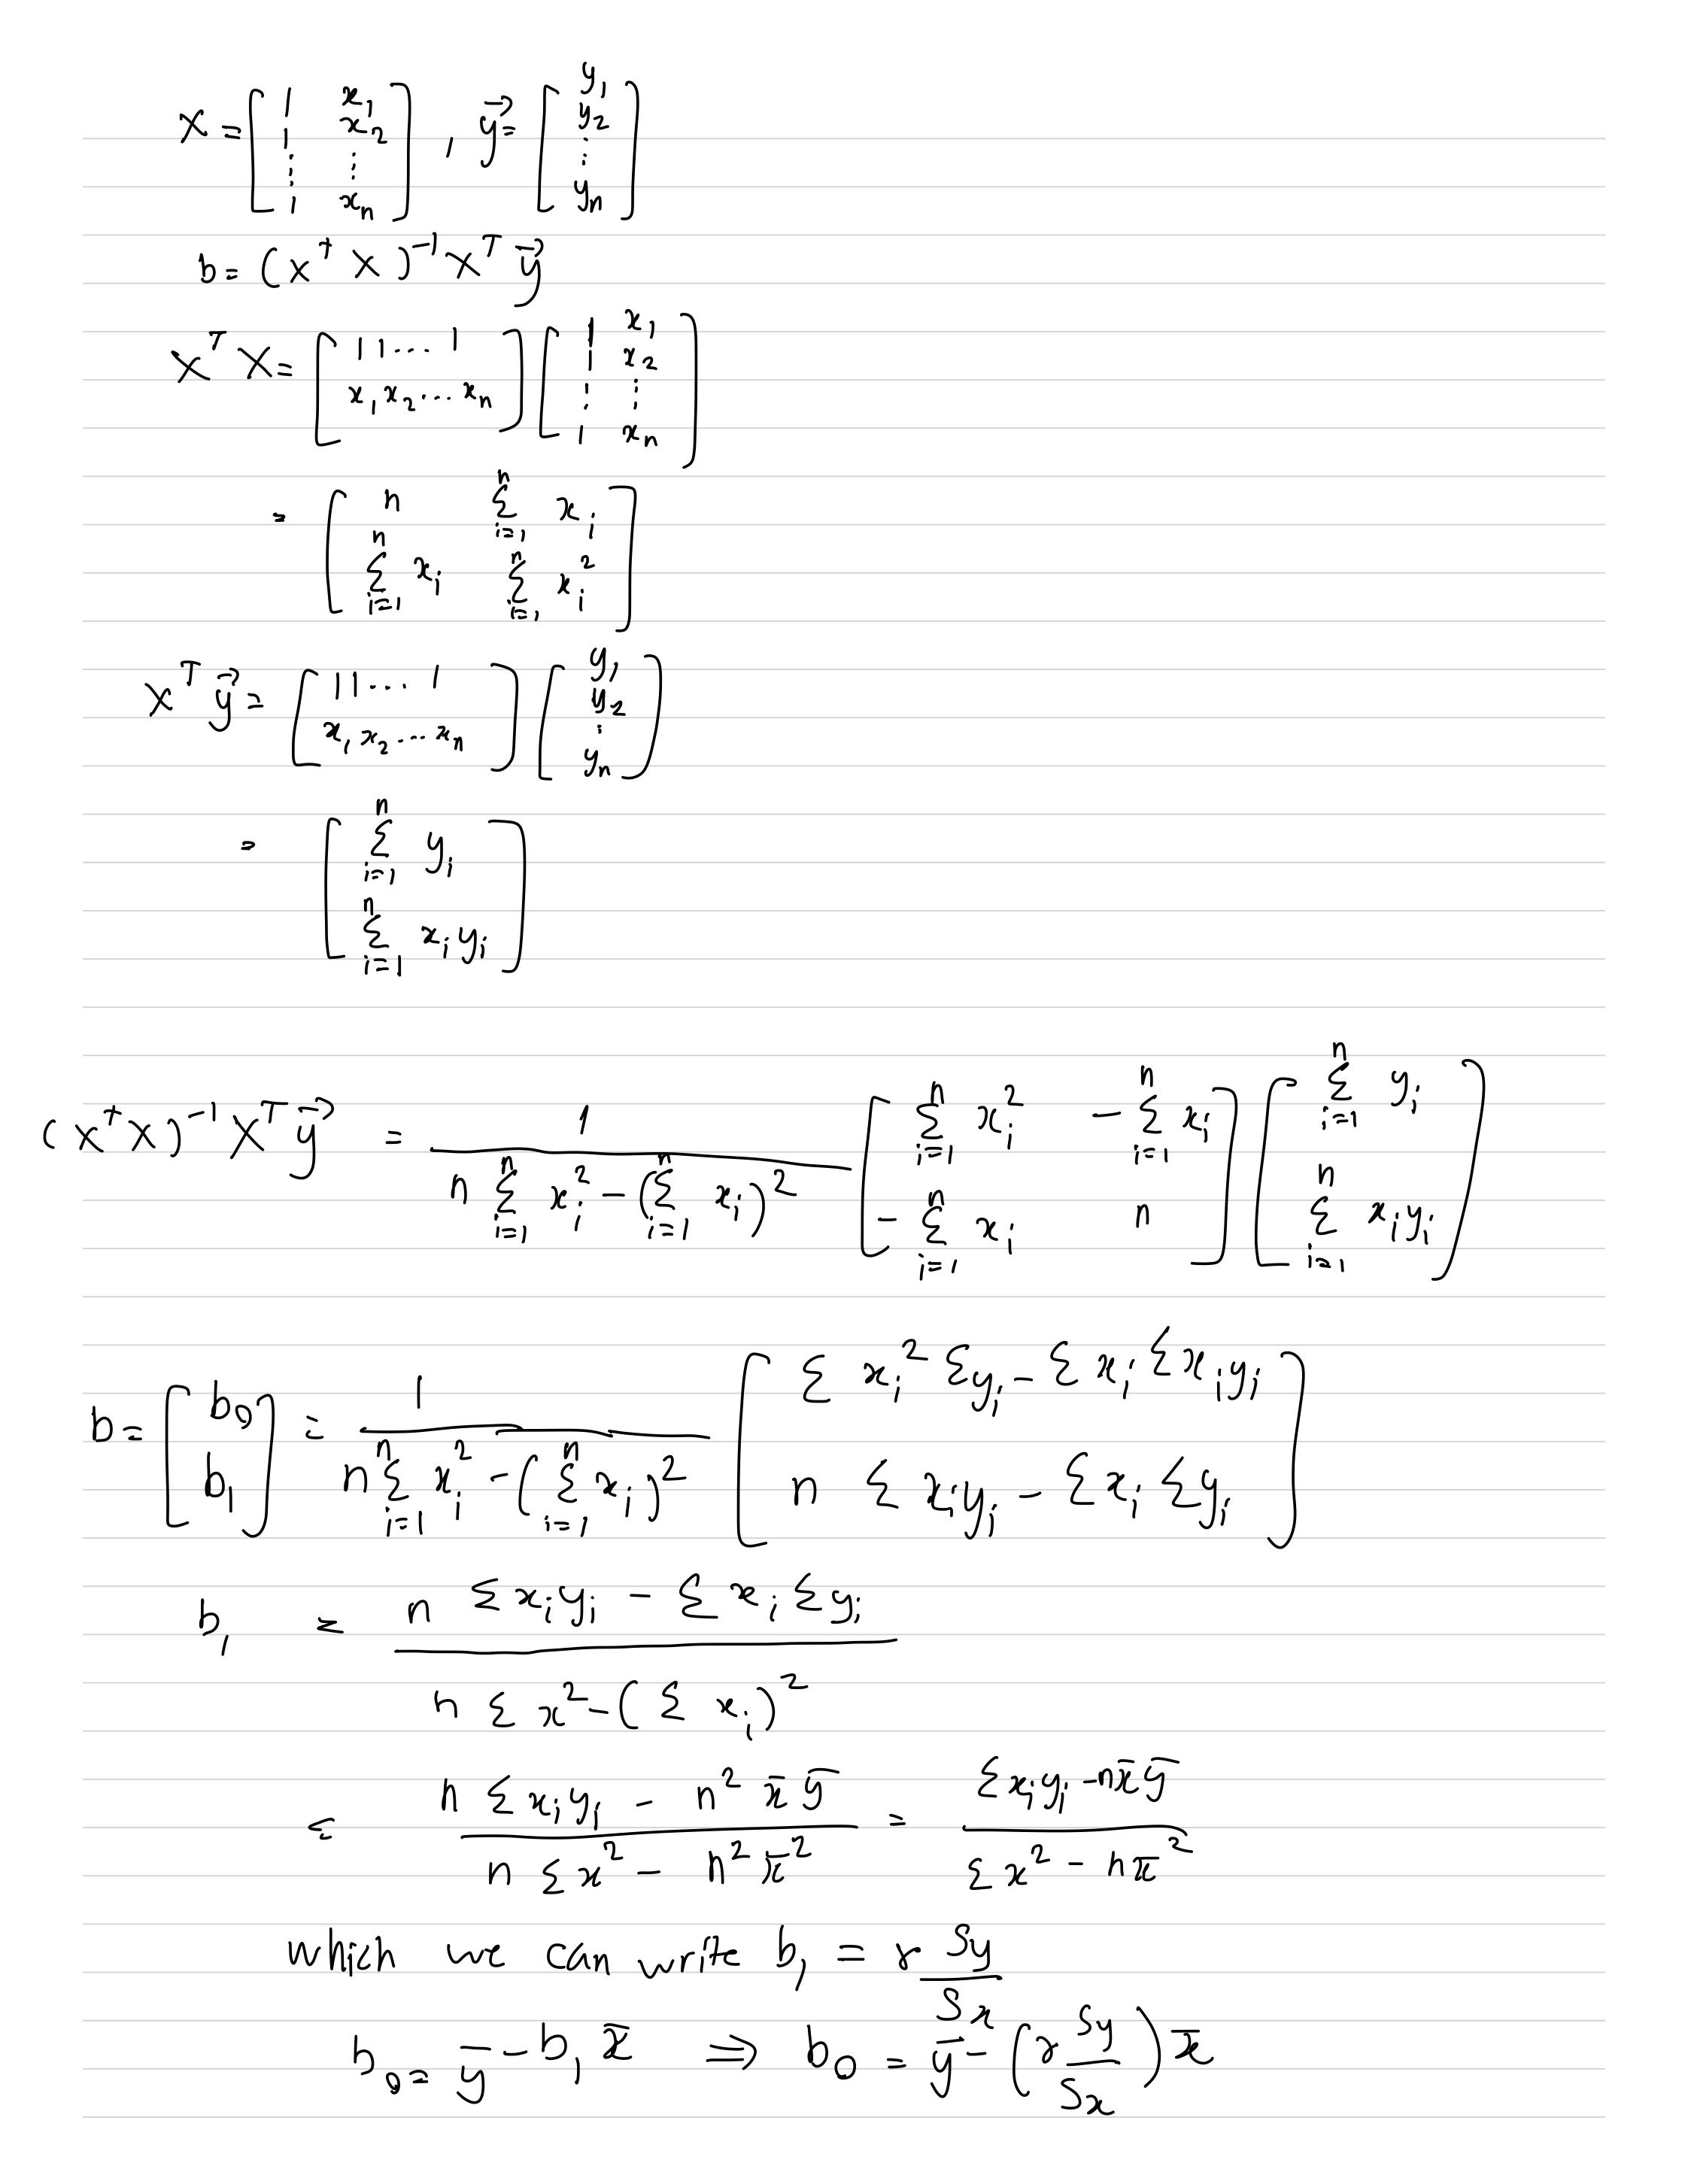
\includegraphics[width=1\linewidth]{hw-11.jpg}
    \caption{Problem 6(c)}
    \label{fig:enter-label}
\end{figure}

\easysubproblem{If $X$ is rank deficient, how can you solve for $\b$? Explain in English.} \spc{2}

If $X$ is rank deficient which means it has linearly dependent columns or duplicate features, we cannot find the inverse since it is not full rank and it is not invertible. So, we need to drop the duplicate feature or linearly dependent columns to be able to find the inverse.

\hardsubproblem{Prove $\rank{X} =\rank{X^\top X}$.}\spc{9}

%\hardsubproblem{Given matrix $X \in \reals^{n \times (p+1)}$, full rank and first column consisting of the $\onevec_n$ vector, now consider cost multiples (\qu{weights}) $c_1, c_2, \ldots, c_n$ for each mistake $e_i$. As an example, previously the mistake for the 17th observation was $e_{17} := y_{17} - \hat{y}_{17}$ but now it would be $e_{17} := c_{17} (y_{17} - \hat{y}_{17})$.  Derive the weighted least squares solution $\b$. No need to rederive the facts about vector derivatives. Hints: (1) show that SSE is a quadratic form with the matrix $C$ in the middle (2) Split this matrix up into two pieces i.e. $C = C^{\half} C^{\half}$, distribute and then foil (3) note that a scalar value equals its own transpose and (4) use the vector derivative formulas.}\spc{10}


\intermediatesubproblem{[MA] If $p=1$, prove $r^2 = R^2$ i.e. the linear correlation is the same as proportion of sample variance explained in a least squares linear model.}\spc{6}

\intermediatesubproblem{Prove that $g(\bracks{1 ~\xbar_1~ \xbar_2~ \ldots~ \xbar_p}) =\bar{y}$ in OLS.}\spc{7}


\[
g(\mathbf{x}) = \mathbf{x}^\top \mathbf{b}
\]


\[
g(\bar{\mathbf{x}}) = \bar{\mathbf{x}}^\top \mathbf{b}
\]



\[
\bar{\mathbf{x}} = \frac{1}{n} \sum_{i=1}^{n} \mathbf{x}_i,
\]


\[
g(\bar{\mathbf{x}}) = \left( \frac{1}{n} \sum_{i=1}^{n} \mathbf{x}_i \right)^\top \mathbf{b} = \frac{1}{n} \sum_{i=1}^{n} \mathbf{x}_i^\top \mathbf{b}.
\]


\[
g(\mathbf{x}_i) = \mathbf{x}_i^\top \mathbf{b},
\]


\[
g(\bar{\mathbf{x}}) = \frac{1}{n} \sum_{i=1}^{n} g(\mathbf{x}_i).
\]


From OLS properties, the sum of residuals is zero:

\[
\sum_{i=1}^{n} (y_i - g(\mathbf{x}_i)) = 0.
\]

\[
\sum_{i=1}^{n} y_i = \sum_{i=1}^{n} g(\mathbf{x}_i).
\]



\[
\bar{y} = \frac{1}{n} \sum_{i=1}^{n} g(\mathbf{x}_i).
\]


\[
g(\bar{\mathbf{x}}) = \bar{y}.
\]



\intermediatesubproblem{Prove that $\bar{e} = 0$ in OLS.}\spc{10}

\hardsubproblem{If you model $\y$ with one categorical nominal variable that has levels $A, B, C$, prove that the OLS estimates look like $\ybar_A$ if $x = A$, $\ybar_B$ if $x = B$ and $\ybar_C$ if $x = C$. You can choose to use an intercept or not. Likely without is easier.}\spc{10}


\intermediatesubproblem{[MA] Prove that the OLS model always has $R^2 \in \zeroonecl$.}\spc{5}

\end{enumerate}



\end{document}

